% !TeX encoding = UTF-8
\documentclass[12pt,a4paper]{article}

% 未翻译完时使用方便标注中文
%\usepackage{ctex}

% 使用字体 palatino
%\usepackage{palatino}

% 颜色宏包
\usepackage{xcolor}
% 抄录环境
\usepackage{verbatim}

% 数学宏包
\usepackage{amsmath,amssymb,amstext}
\usepackage{mathrsfs}
\usepackage{array}
\usepackage{latexsym}
\usepackage{leftidx}
\usepackage{algorithm}
\usepackage{algpseudocode}
% The package provides a command \syntaxonly that
% suppresses output from a LATEX run.c
\usepackage{syntonly}

% 插图
\usepackage{graphicx}
\usepackage{subfigure}
\usepackage{caption}

% 浮动宏包,H选项将图形, 表格位置固定
\usepackage{float}

% 获取最后一页页码
\usepackage{lastpage}

% 三线表, 长表格, 复杂表格
\usepackage{tabularx}
\usepackage{booktabs}
\usepackage{longtable}
\usepackage{multirow}
\usepackage{bigstrut}

% 表格颜色宏包
\usepackage{colortbl}

% 超链接设置
\usepackage[
pdfstartview=FitH,
bookmarks=true,
bookmarksnumbered=true,
bookmarksopen=true,
linkcolor=black,
citecolor=black,
pagecolor=black,
colorlinks=true,
pdfborder=001,
linkcolor=black,
citecolor=black,
urlcolor=black
]{hyperref}

% 页边距宏包
\usepackage{geometry}
\geometry{left=1.2in,right=1.2in,top=2.5cm,bottom=2.5cm}

% 页眉, 页脚设置
\usepackage{fancyheadings}
\usepackage{fancyhdr}
\pagestyle{fancy}
\fancyhead{} % clear all header fields
\fancyfoot{} % clear all footer fields
\setlength{\headwidth}{\textwidth}
% 队号
\lhead{\footnotesize{Team{} \#{} 10086}}
\chead{}
\rhead{\footnotesize{Page{} \thepage{} of{} \pageref{LastPage}}}
\renewcommand{\headrulewidth}{0.4pt}

% 枚举环境
\usepackage{enumitem}
\setenumerate[1]{itemsep=5pt,partopsep=0pt,parsep=\parskip,topsep=5pt}
\setitemize[1]{itemsep=5pt,partopsep=0pt,parsep=\parskip,topsep=5pt}

% 行间距
\linespread{1}
% 段间距
\setlength{\parskip}{0.5\baselineskip}
% 修改文字与标题距离
\setlength{\abovecaptionskip}{2pt plus2pt minus 1pt} %
\setlength{\belowcaptionskip}{2pt plus2pt minus 1pt} %


% 定义字体 myfonta, myfontb
\DeclareFixedFont{\myfonta}{OT1}{ugq}{b}{n}{20pt}
\DeclareFixedFont{\myfontb}{OT1}{ugq}{b}{n}{20pt}

% 定义图片, 表格, 公式引用命令(也可以直接用\ref, 但不是很好看)
\newcommand*{\figref}[1]{{\bf Figure~\ref{#1}}}
\newcommand*{\tabref}[1]{{\bf Table~\ref{#1}}}
\newcommand*{\equref}[1]{{\bf Equation~\eqref{#1}}}

% 设置一个插图存放目录
\graphicspath{{figures/}}
\begin{document}
\footnotesize
\begin{center}
    \begin{minipage}[c]{0.3\textwidth}
        \baselineskip=1.4\baselineskip
        \flushleft
        \begin{tabbing}
            For office use only\\
            T1\underline{\makebox[32.5mm][c]{}}\\
            T2\underline{\makebox[32.5mm][c]{}}\\
            T3\underline{\makebox[32.5mm][c]{}}\\
            T4\underline{\makebox[32.5mm][c]{}}
        \end{tabbing}
    \end{minipage}\qquad\qquad
    \begin{minipage}[c][3.5cm]{0.3\textwidth}
        \begin{center}
            Team Control Number
            \vfill
            % 队号
            {\myfonta{10086}}
            \vfill
            \vfill
            Problem Chosen
            \vfill
            % 选题
            \myfontb{B}
        \end{center}
    \end{minipage}\qquad\qquad
    \begin{minipage}[c]{0.3\textwidth}
        \baselineskip=1.4\baselineskip
        \flushright
        \begin{tabbing}
            For office use only\\
            F1\underline{\makebox[32.5mm][c]{}}\\
            F2\underline{\makebox[32.5mm][c]{}}\\
            F3\underline{\makebox[32.5mm][c]{}}\\
            F4\underline{\makebox[32.5mm][c]{}}
        \end{tabbing}
    \end{minipage}
\end{center}

\bigskip
\vspace{-0.7cm}
{\noindent\color{gray}\rule[0.25\baselineskip]{\textwidth}{1.5pt}}

\thispagestyle{empty}

\vspace{-0.7cm}
\begin{footnotesize}
    %\begin{center}
        % Summary 说明
    %    \bf{2014 Mathematical Contest in Modeling (MCM) Summary Sheet}\\
    %\end{center}

    \begin{center}
        \textbf{Summary}
    \end{center}
        % Summary 正文
\par
In our paper, we focus on addressing problems of water quality forecast and the building of the lake’s evaluation system. Then we apply them into Chao Hu. Lastly, we analyze the results, meanwhile, putting forward suggestions on the improvement of the land management.\par
First and foremost, this paper mainly places emphasis on the nitrogen and phosphorus input as the criterion of lake, then a model for predicting water quality can be divided into two sections. We formulate an export coefficient model accounting for factors influencing the output of N and P in order to estimate and forecast nitrogen and phosphorus load under the different land use. On the basis of obtaining N and P outputs, BP neural network model is built by combining with indictors as inputs like temperature, PH and so on to predict potentially-toxic algal blooms. To ground this model in reality, we incorporate 91 groups data collected from the websites for train and 19 groups data used for the simulation. The simulation results agreeing well with real situation indicate that the model is efficient and reliable.\par
Secondly, a strategy based on analytic hierarchy process is proposed to build lake evaluation model. We collect the values of seven indexes judging lakes through local knowledge and expertise. Then we use AHP to determine the weight of seven factors and finally evaluate Chao Hu successfully. We draw conclusion that Chao Hu lies inⅢ,middle level.\par
Eventually, the sensitivity analysis of the evaluation model is carried out to ensure the utility. It is found that the model is shortage of insufficient stability by analyzing the sensitivity of environmental awareness, for lakes evaluation is a complicated system and cannot be described by simple indexes. So the model need to be improved.\par
\end{footnotesize}


\newpage
\thispagestyle{fancy}
\newpage
\setcounter{page}{1}
\vspace{2cm}

%\begin{center}
%    \begin{normalsize}
%Abstract Title
%    \end{normalsize}\\
%\end{center}

\begin{abstract}
    \begin{footnotesize}{}
% Abstract 正文
In our paper, we focus on addressing problems of water quality forecast and the building of the lake’s evaluation system. Then we apply them into Chao Hu. Lastly, we analyze the results, meanwhile, putting forward suggestions on the improvement of the land management.\par
First and foremost, we build a model to predict the water quality and potentially-toxic algal blooms. We divide the model into two sections. The first is the Export Coefficient Model, which is used to estimate and forecast nitrogen and phosphorus load under the different land-use. On the basis of obtaining N and P outputs, BP neural network model is built by combining with indictors as inputs like temperature, PH and so on to predict potentially-toxic algal blooms. To ground this model in reality, we incorporate 91 groups data collected from the websites for train and 19 groups data used for the test. The data of Chao Hu are used for simulation. The simulation results agree well with real situation indicating that the model is efficient and reliable.\par
Secondly, we build the lake evaluation model based on analytic hierarchy process. We collect the values of seven indexes judging lakes through local knowledge and expertise. Then we use AHP to determine the weight of seven factors and finally evaluate Chao Hu successfully. We draw conclusion that Chao Hu lies in Ⅲ,belonging to middle level.\par
Eventually, the sensitivity analysis of the evaluation model is carried out to ensure the utility. It is found that the model is shortage of insufficient stability by analyzing the sensitivity of environmental awareness, for lakes evaluation is a complicated system and cannot be described by simple indexes. So the model need to be improved.\par
    \end{footnotesize}
\end{abstract}



\newpage
\tableofcontents
\newpage

\section{Introduction}
%1.1巢湖现状
\subsection{Present situation of Chao Hu}     
%巢湖位于安徽省中部,长江北岸,流域面积达 1.35 万平方公里.流域地形以丘陵、平原为主.巢湖流域河网密集,环湖河流成向心状分布,湖泊、 水库、 渠塘及水田等广泛分布.随着巢湖流域人口和工农业生产的快速增长,需水量和污水排放量增大,相应地增加了入湖污染量.农业活动、 土地利用等造成巢湖水体氮、 磷等营养负荷加重,湖泊生态恶化,非点源污染问题较为突出.
Chao Hu is located in the central An Hui Province, at north bank of the Yangtze River, whose basin area comes up to 13500 square kilometers. Watershed topography mainly consists of hills and plains. The key rivers surrounding the Chao Hu where the densities of river net are high take on centripetal selection distribution, what's more, lakes, reservoirs and paddy fields are widely dispersed. With the rapid growth of population and industrial production around Chao Hu catchment, water demand and wastewater discharge increase gradually, correspondingly rendering more sewage to be drained to lakes. Agricultural activities and unreasonable land use give birth to weight the load of nitrogen and phosphorus concentrations in water, inevitably, accelerating the lake ecosystem's deterioration. Especially, non-point source pollution problem is more prominent.\par

\subsection{Previous research}
%20 世纪 90 年代, 巢湖流域非点源污染及由此引起的巢湖生态环境问题逐渐引起人们关注.张之源,王培华等根据 1986 年 - 1995 年近 10 年的巢湖水质监测数据, 得出非点源 TN 负荷平均占总量的 49% ,TP 占 40% ,同时探讨了污染物的湖内空间分布.该阶段对巢湖流域的非点源污染来源、 特征及管理控制等问题未作出系统研究,属于初步调查阶段.王宗志等在上述研究基础上利用模糊聚类方法分析巢湖流域几种污染物的主要来源,进而得到11种土地利用方式与营养物输出浓度间的对应关系.
The potential impact of no-point source pollution on Chao Hu ecosystem raises widely concern in the early 1990s, Zhang Zhi Yuan and Wang Pei Hua reported that no-point source on the average of TN load account for 49\% of the total, and TP is about 40\%, meanwhile, discussing the spatial distribution of pollutants in water according to the monitoring data of Chao Hu from 1986 to 1985. However, the initial research phase did not involve the major source of no-point source pollution, effects of different management scenarios on the lake and administrative console problems. Wang Zong Zhi exploited fuzzy clustering method to analyze the major source of several pollutants in the Chao Hu basin, thereby gaining the relationship between eleven land use patterns and nutrient outputs. Here, we focus on the need for solving the problem about linking different domains influencing pollutants input and also forecasting and evaluating the effects of different management scenarios on lakes.\par

\subsection{Outline of our model}
%在我们的论文中,我们首先将巢湖流域内的土地分为8种类型,建立输出系数模型,求出各个类型土地N、P的负荷,分析巢湖水质问题;然后,结合气象学、其他水系影响等因素,对巢湖赤潮发生进行预测;最后,建立基于层次分析法的评价模型,建立六个评价级别,利用搜集数据,对巢湖做出评价.\par
Firstly we divide the land into nine type in our paper. Then we build the Export Coefficient Model to get the load of N and P. Given the amount of N and P, we analyze the water quality. Next combining the meteorology and the other factors, we forecast the potentially-toxic algal blooms. Lastly, we building the evaluation model based on the AHP. What's more, we create an evaluation system. We can evaluate the Chao Hu with the evaluation model and evaluation system.\par

\section{Problem Restatement and Analysis}
\subsection{Problem Restatement}
%首先,题目告诉我们,湖泊提供的商品和服务是由于气象、水文地理、营养物质负荷以及其他注入湖泊等因素之间相互作用的产物.而且还说明,水文地理和营养物质负荷是受到社会经济的影响,例如人类居住、抽引水、土地管理等.然后题目要求,建立合适的模型,将不同的领域联系起来,并且要求对湖泊进行评价和预测.\par
Firstly, from the question we can know that the goods and services that lakes provide result from complex interactions between meteorology, hydrology, nutrient loads and in-lake processes. In addition, we know that Hydrology and nutrient loads are, in turn, influenced by socio-economic factors such as human habitation, water abstraction and land-management, within their catchments. The last, the question let us build models to link these different domains and forecast the effects of different management scenarios on lakes and evaluate the lake.\par

\subsection{Problem Analysis}
%湖泊水质和赤潮发生情况是评价它的重要标准.而影响湖泊水质的主要指标是不同土地类型的N、P负荷.对于水质的预测,我们可以建立土地类型与N、P负荷之间联系的模型来解决问题.\par
In order to build a model for forecasting the effects of different land management scenarios on lakes, we find that the reason for which land management can have great impacts on lakes is that different land use contributes different nitrogen and phosphorus concentrations which are the criterion of  water quality to Chao Hu, apparently, we can formulate model based on the relationships between land management and nitrogen, phosphorus load to forecast the water quality. Besides land management, we cannot ignore the effects of temperature, hydrology and meteorology on the output of nitrogen and phosphorus.\par
Furthermore, nitrogen and phosphorus loads are closely related to potentially-toxic algal blooms. The number of algal blooms can be represented by chlorophyll, so the neural network can be built by chlorophyll as output and factors influencing potentially-toxic algal blooms reproduction as inputs to forecast the water quality indirectly.\par
Eventually, we could get data about nitrogen and phosphorus concentrations with chlorophyll, then a six-level evaluation system can be established combined with factors affecting the above data by AHP algorithm.\par

%查阅相关文献资料,我们了解到,水域内藻类的数量可以用叶绿素A来表征,而且当叶绿素A的含量高于0.01mg/L时,表明水域藻类数量达到了发生赤潮的条件.赤潮是一种复杂的生态异常现象,发生的原因也比较复杂,所以,我们建立神经网络模型,对可能影响赤潮发生的因素作为输出,叶绿素A含量作为输出,从而对水域赤潮的发生进行预测. 
%在论文中,根据题目要求,我们还需要建立湖泊的评价模型.我们建立了基于层次分析算法的评价模型.其中,最上层是湖泊综合评价.中间层是N、P总量和叶绿素A含量.土地管理方案、温度、PH值、含氧量构成最下层.然后,我们根据文献资料,建立一个包含六个级别的评价体系.最后,结合数据就可以对巢湖进行评价并判断级别.

\section{General Assumptions}
\begin{itemize}
    %1.	假设收集的数据准确可靠,能够较好的反映真实情况;
    \item Assuming that data collected is accurate and reliable, and can reflect real conditions preferably.
    %2.	假设我们自己设定的几种不同的土地管理方案,各种类型土地的输出系数只与类型有关,与该类型面积大小及其他因素无关;
    \item The different land use management scenarios were formulated in order to improve models' applicability, moreover, nutrient export coefficients from land are only subject to land use types, not its area and so on.
    %假设改变不同类型土地的比例时,温度、降雨量等因素保持相同.
    \item Temperature, rainfall runoff and other factors which affect Nitrogen and Phosphorus concentrations in soil drained to Chao Hu should be at the same rate when we change the proportions of different land use.      
    %假设污染物质量守恒
    \item Under a certain scope, pollutants from agricultural fertilizer, septic tank, industrial plant and so on do not change with time and obey conservation law of mass.
\end{itemize}\par

%4 不同土地管理方案对湖泊影响的预测模型
\section{Forecasting models about effects of different management scenarios on lakes}
%不同的土地管理方案,会影响湖泊的TN负荷和TP负荷,从而影响水质.而且,当水中N、P含量超标时,加上合适的温度等其他条件,就会发生赤潮现象.湖泊水质会更加恶化.所以,我们首先建立对N、P含量的估算和预测模型.然后是是否发生赤潮的预测模型.
Different land use managements will have an impact on TN and TP load in lakes,
moreover, water containing elevated level of N,P with proper temperature and other factors precipitate potentially-toxic algal blooms reproduction, to some extent, making water quality severely worse. Firstly, we establish a model to estimate nitrogen and phosphorus concentrations and forecasting model for water quality which lay a firm foundation for evaluation model.\par

%4.1  N、P量估算与预测的输出系数模型
\subsection{Estimation of N,P concentrations and Export Coefficient Model}

%4.11  模型介绍
\subsubsection{Introduction to models}
%研究土地利用-营养物质-湖泊富营养化关系的过程中,提出并应用了输出系数模型(也称单位面积负荷法).模型在考虑土地利用分类的基础上,结合居民非点源污染物的排放和处理、牲畜的数量和分布来确定不同污染源的输出系数.同时模型在对总氮进行估算时还考虑了植物的固氮、氮的空气沉降等因素.该模型能较为准确的对大尺度流域的非点源污染进行评价和预测.模型的一般表达式为:
Researchers put forward and apply export coefficient model in the process of studying the relationships between nutrient and lake eutrophication.$^{[\ref{1}]}$On the basis of considering land use management, we can determine export coefficients of different pollutants by combining the emission of no-point pollutants and the number and distribution of livestock. At the same time, the model also accounts for factors about nitrogen fixation in plants and air precipitation of nitrogen. The model is applicable in forecasting and evaluating no-point polluted catchment with big scale. The general expression of model is that:

\begin{equation}L_i=\sum_{j=1}^nE_{ij}A_j+p\end{equation}

%其中,$i$为污染物类型.$j$为流域中营养源的种类,共$n$种.$L_i$为污染物i在流域的总负荷量.$E_{ij}$为污染物$i$在流域第j种营养源的输出系数.$A_j$为第$j$种营养源的数量.$p$为由降雨输入的营养物数量.\par
In the equation, $i$ refers to the type of pollutant,j refers to the kind of nutrient source. $L_i$ refers to the total loads of pollutant $i$. $E_ij$ refers to the export coefficient of $i$ pollutant exporting $j$ nutrient source. $A_j$ refers to the number of $j$ nutrient source, p refers to the number of nutrient source due to raining.\par

%输出系数模型利用黑箱原理,避开了非点源污染发生的复杂过程,所需参数少,操作简单,且具有一定的精度,在国内外得到了广泛的应用.
Export coefficient models exploit principles of black box, avoiding the complicated progress which no-point pollution may happen, and it has a certain accuracy. \par

%4.12  模型参数的确定方法
\subsubsection{The methods of determining model's parameters}
%在应用输出系数模型时,关键问题是确定合理的输出系数值.在明确的土地利用情况的基础上,获取输出系数的常用途径是现场监测和查阅文献值.两种方法的比较如下表:
The key to solve problem is to determine a reasonable output coefficient when applying export coefficient model, on the basis of land use condition, the way to acquire export coefficient is field inspection and consulting literature. We will proceed them as follows:

\begin{figure}[H]
\centering
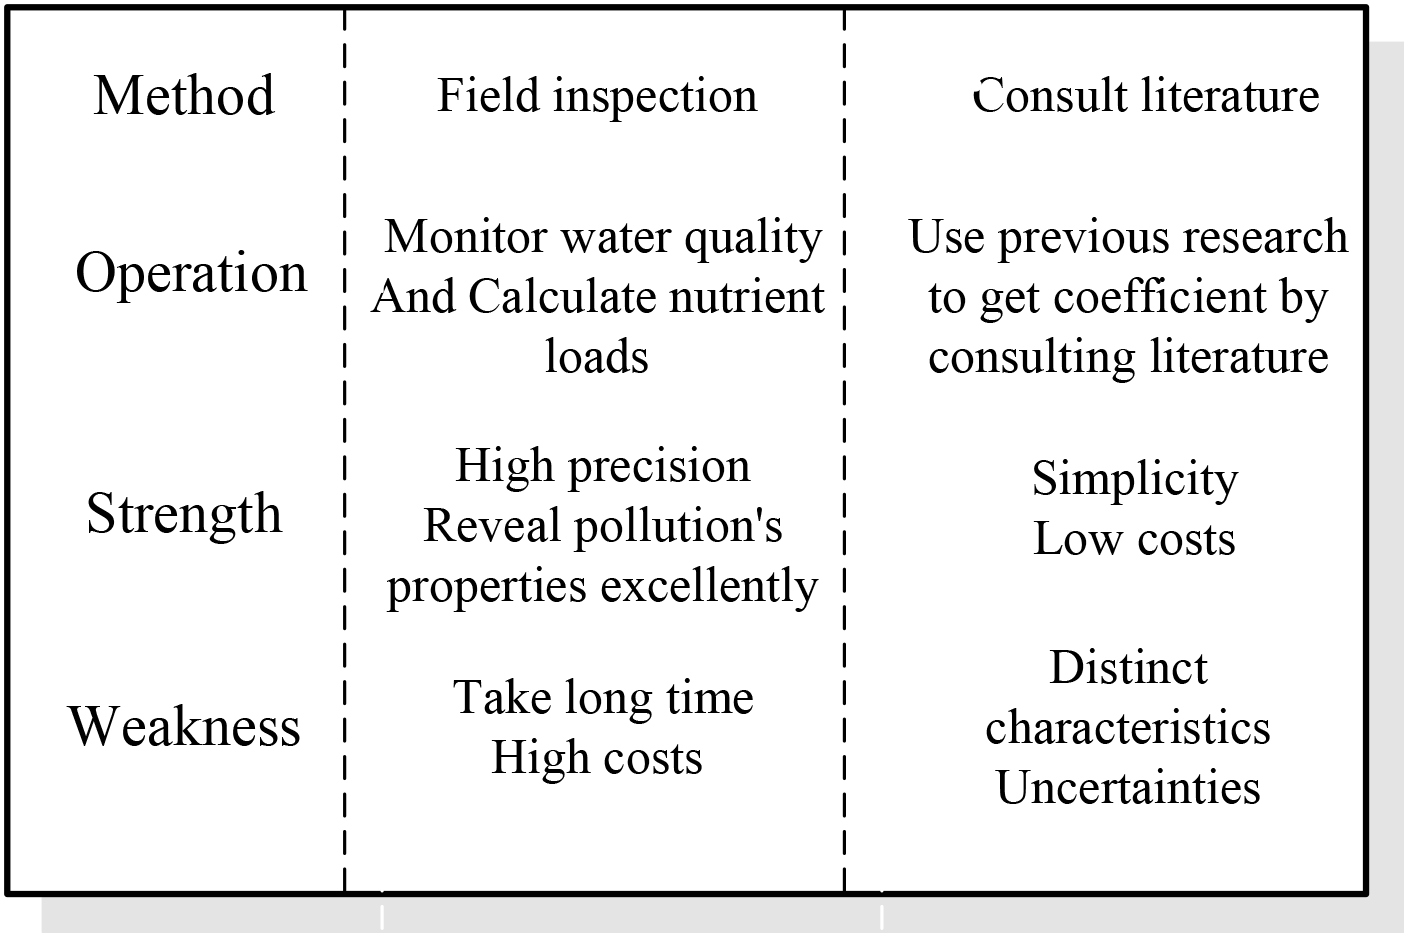
\includegraphics[width=0.7\linewidth]{figure/13}
\caption{\footnotesize {Symbols Used in This Section}}
\end{figure}

%\begin{table}[H] 
%    \begin{center}
%        \caption{\footnotesize {Symbols Used in This Section}}
%        \begin{footnotesize}
%            \begin{tabularx}{\textwidth}{|c|c|c|}
 %               \hline
  %              Method & Field inspection & Consult literature \\
   %             
    %            Operation & Monitor water quality  Calculate nutrient loads & Use previous research to get coefficient by consulting literature \\
     %           
      %          Strength & High precision Reveal pollution's properties excellently & Simplicity Low costs \\
       %         
        %        Weakness & Take long time High costs & Distinct characteristics Uncertainties\\
         %       \hline           
          %  \end{tabularx}%
        %\end{footnotesize}
    %\end{center}
%\end{table}
\vspace{-1cm}


%\subsubsection{基于水文水质资料的输出系数确定法的模型建立}
\subsubsection{Determine export coefficients based on hydrological materials}
%在输出系数中,受地域影响最大的是土地利用的输出系数.本文尝试在污染物质量守恒的前提下,采用基于历史水文水质监测资料的确定各土地类型的输出系数的方法.该方法兼具了现场监测和查阅文献两种方法.它比较适合我国缺乏非点源污染监测资料的现状.具体建模过程如下:
Area has the greatest impacts on the land use coefficient. under the premise of the law conservation of mass, we determine the different land export coefficients taking advantage of monitoring data, which is applicable in present situation being shortage of no-point pollution data.\par

\begin{itemize}
    %Step1土地利用的分类与小流域选取
    \item  Classifying land use and selecting small watershed \\
    %根据研究的精度需要,将土地利用分为n种类型.在研究区内选取m个小流域,根据污染物在流域内输入输出质量守恒原则,建立产污方程:
    The land use is divided into n types according to research,then selecting m small watersheds,pollutants' inputs and outputs obey the law conservation of mass, we get   
    
    \begin{equation}L_i=L_{ps}+L_{io}+\sum_{j=1}^n[E_{ij}(M_{ij})]A_j+p\end{equation}
    
   \newpage
    %Step2求解参数Li
    \item   Solving parameter $L_i$ \\
    
    \begin{equation}L_i=C_i\times\frac{Q}{k_i}\end{equation}
    
    %其中,$C_i$为小流域出口第$i$种污染物的年平均监测浓度. $Q$为流域出口的年总流量.$ki$为第$i$种污染物在小流域的损失系数.$K_i$的量纲为“1”.
    $C_i$ refers to the average of $i$ pollutant of monitoring concentrations a year.$Q$ refers to annual flow.
    %Step3求解参数Lps和Lio
    \item  Geting parameter about $lps$ and $lio$
    %据式(2)和式(3),可得:
    According to \equref{2} and \equref{3},we have
    
    \begin{equation}\frac{C_i\times Q}{k_i}=L_{ps}+L_{io}+\sum_{j=1}^n[E_{ij}(M_{ij})]A_j+p\end{equation}
    
    %其中,$L_{ps}$表示农村生活,$L_{io}$表示畜禽养殖;
    $L_{ps}$ refers to country life, $L_{io}$ refers to the breeding of livestock
    \begin{equation}L_{ps}=\frac{C_k\times Q_k}{D_k\times k_i}\end{equation}
    
    %式中:$C_i$枯为枯水期流域出口第$i$种污染物的平均监测浓度.$Q$枯为枯水期流域出口的总流量.$D$枯为枯水期的时间.
    $C_k$ refers to the average of i pollutant of monitoring concentrations. $Q_k$ refers to total flows during dry season.$D_k$ refers to the time of dry season.
    
    %公式6
    \begin{equation}L_{io}=\sum_{j=1}^{n}[E_{ij}M_{ij}]A_j\end{equation}
    
    %式中,$i$为污染物类型;$j$为人或畜禽类型;$L_{io}$为第i种污染物总负荷. $E_{ij}$为单位数量第$j$种污染源第$i$种污染物的输出数(该值来自文献);$M_{ij}$为第$j$种污染源的第$i$种污染物的营养物输入量$A_j$为人口数或畜禽养殖量.
    $i$ refers to pollutant types, $j$ refers to types of livestock,$E_{ij}$ refers to the number of i th pollutant exporting to $j_{th}$ pollution source in units.
    $M_{ij}$ refers to the nutrient of $i_{th}$ pollutant exporting to $j_{th}$ pollution  source.
    
    %Step4联立方程组求解Eij
    \item Getting solution by a set of simultaneous equations.\\
    %对于污染物$i$,$m$个小流域课得到$m$个产污方程.因此可得到方程组:
    For pollutant $i$, then we have
    
    %公式7
    \begin{equation}
    \begin{cases}
    \displaystyle\frac{C_{i1}\times Q_1}{k_{i1}}=\displaystyle\frac{C_{k1}\times Q_{k1}}{D_{k1}\times k_{i1}}\times365+L_{io1}+\sum_{j=1}^n[E_{ij}(M_{ij})]A_{j1}+p_1\\
    \qquad\qquad\qquad\qquad \qquad\qquad\cdots\\
    \displaystyle\frac{C_{it}\times Q_t}{k_{it}}=\displaystyle\frac{C_{kt}\times Q_{kt}}{D_{kt}\times k_{it}}
    \times365+L_{iot}+\sum_{j=1}^n[E_{ij}(M_{ij})]A_{jt}+p_t\\
    \qquad\qquad\qquad\qquad \qquad\qquad\cdots\\
    \displaystyle\frac{C_{im}\times Q_m}{k_{im}}=\displaystyle\frac{C_{km}\times Q_{km}}{D_{km}\times k_{im}}
    \times365+L_{iom}+\sum_{j=1}^n[E_{ij}(M_{ij})]A_{jm}+p_m
    \end{cases}
    \end{equation}
    
\end{itemize}\par

%4.2  基于BP神经网络的赤潮预测模型
\subsection{Forecasting model based on BP neural network}
%4.21输入输出因子的选取
\subsubsection{The selection of output and input factors}
%由于研究对象的特殊性,我们只能通过各类网站及报告获取到零碎的数据,经过数据规整化后,我们获得了129组数据,由于水体叶绿素a浓度是表征水体中藻类现存量的最直接指标,故水体中总叶绿素a浓度是模型的输出因子,通过对叶绿素a浓度的预测可以间接实现对藻类引发的水华进行预测..在确定模型输出因子后,合理选择网络的输入因子对正确应用BP模型和保证模型预报精度非常重要.因为输入因子中,可能存在与输出因子关联弱的噪声因子,或者重叠反映系统信息的冗余因子.无论是噪音因子还是冗余因子,都会加大分析问题的难度,增加模型的复杂性,最终影响模型预测能力.筛选BP神经网络输入因子的基本原则是选择与输出因子相关而又彼此无关的环境因子网络结构.
In view of particularity of studying object, we get 129 groups data processed which are from all kinds of web sites and papers. The reason why the potentially-toxic algal blooms reproduction can be predicted indirectly via forecasting the content of chlorophyll is that the total content of chlorophyll a is the most direct index to represent the quantity of algal blooms. After determining the output factor, reasonable selection of network‘s input factors is of great importance to apply BP neural network models accurately and guarantee the precision of the model, for input factor may exist noise factor related to outputs and redundant factor reflecting system information. Either of the two conditions will add complexity to model and difficulty to analyze problem so as to affect the predictive ability of model. The principle of sorting out input factors of neural network is to select environment factors of network structure which have nothing to with outputs.\par
%最终,我们以N,P输入总量作为输入因子,去除了数据量过少的因子以及其他可能的噪声因子及冗余因子.
At last, we regard N,P input totals as input factors and get rid of factor lacking data and noise factor and redundant factor.\par

%4.22网络结构
\subsubsection{Determine Network structure}
%早有理论证明:3层BP网络,当各层神经元均采用S型函数时,可满足任意复杂的非线性函数拟合逼近问题【7】.
Theoretical proof long before showed that, three BP layers can satisfy any complicated nonlinear function to fit approximation problem when every layer neurons adopt sigmoid function$^{[\ref{2}]}$. The conclusion can provide reference for ensuring algal blooms as three layers network structure, one input layer, one hidden layer and one output layer. Although selecting the number of hidden layer's neurons and activation function between layer and interlayer is regular, the results are even altogether different$^{[\ref{3}]}$.\par  
%这个存在性结论对神经网络结构的设计具有重要的指导作用.参考该结论,确定水华预测模型为3层网络结构,即1个输入层、1个隐含层和1个输出层.然而,选取隐含层神经元数、层与层间的激活函数,虽然有规则可依,但所得结果差异较大,甚至完全不同【8】. 

%4.23隐含层神经元数
\subsubsection{Select neurons of hidden layer}
%通过对不同隐含层神经元数的模型进行训练,使用Mean squared normalized error performance function来分析隐含层神经元数对训练效果的影响,从分析结果发现:当隐含层神经元数大于3个时,训练效果开始随隐含层神经元数的增长在小范围波动,总体上效果很好,当隐含层神经元数为20时,得到最好结果,加上我们的数据集不是很大,因此我们以20作为隐含层神经元数.
Through training neurons of different hidden layers, using mean squared normalized error performance function analyzes the numbers of neurons in hidden layer on the impacts of training effects, then we draw a conclusion from results that training effects fluctuate in a small scale with the increasement of neurons of hidden layer in number when they are more than three. Moreover, we can get the best result when the numbers of neurons are twenty, so we set up twenty neurons as hidden layer considering not many data.\par

%隐含层神经元数
\begin{figure}[H]
\centering
\includegraphics[width=0.7\linewidth]{figure/BestHiddenNeurons}
\caption{Best Hidden Neurons}
\end{figure}\par

%4.24激活函数
\subsubsection{Activation Function}
We set up a sigmoid transfer function in the hidden layer and a linear transfer function in the output layer

%依照上述的网络结构,得到网络结构拓扑以及模型表达式According to the above network structure ,we have network topology and
%y=purelin(V·tansig(W·x+b1)+b2).

\begin{equation}y=purelin(V\cdot tansig(W\cdot x+b_1)+b_2)\end{equation}

%式中:x为输入变量, Y为输出变量,即当前N,P浓度下的叶绿素a浓度;w和b.为输入层与隐含层问连接权重和阈值;y和b.隐含层与输出层间的连接权重和阈值.
In the equation:$x$ represents N,P concentrations and $y$ represents the content of chlorophyll a ,$W$ and $b$ represent link weights between input layer and hidden layer. $Y$ and $b$ represent link weights between hidden layers and output layer. 

%5 基于层次分析法的湖泊评价模型
\section{Evaluation model of lakes based on AHP}
%层次分析法是将定性与定量相结合的系统分析方法.该方法最适宜于解决那些难以完全用定量方法进行分析的决策问题.我们在充分考虑湖泊生态系统实际情况的基础上,从湖泊生态特征、自然功能和社会环境3个方面的评价指标中筛选出7项指标.我们运用层次分析法建立了湖泊的评价模型.
Analytic hierarchy process method is a kind of qualitative and quantitative analysis of multiplicate objective decision, which is applicable in the problem hard to be solved. We sort out 7 indicators from the three aspects of ecological features, native functionality and social environment accounting for the real situation of lake ecosystem to apply in the AHP model.\par

%5.1 模型建立 
\subsection{Construction of AHP Model}
%湖泊评价模型具体建立过程如下:
The process of building evaluation model is as follows
\begin{itemize}
    %建立递阶层次结构模型
    \item Build hierarchical structure \\
    %通过查阅相关资料、文献,我们建立了层次模型,结果如下图所示:
    We build hierarchy model by looking through materials, the result is as follows:

    %层次结构图
    \parbox{\linewidth}{\centering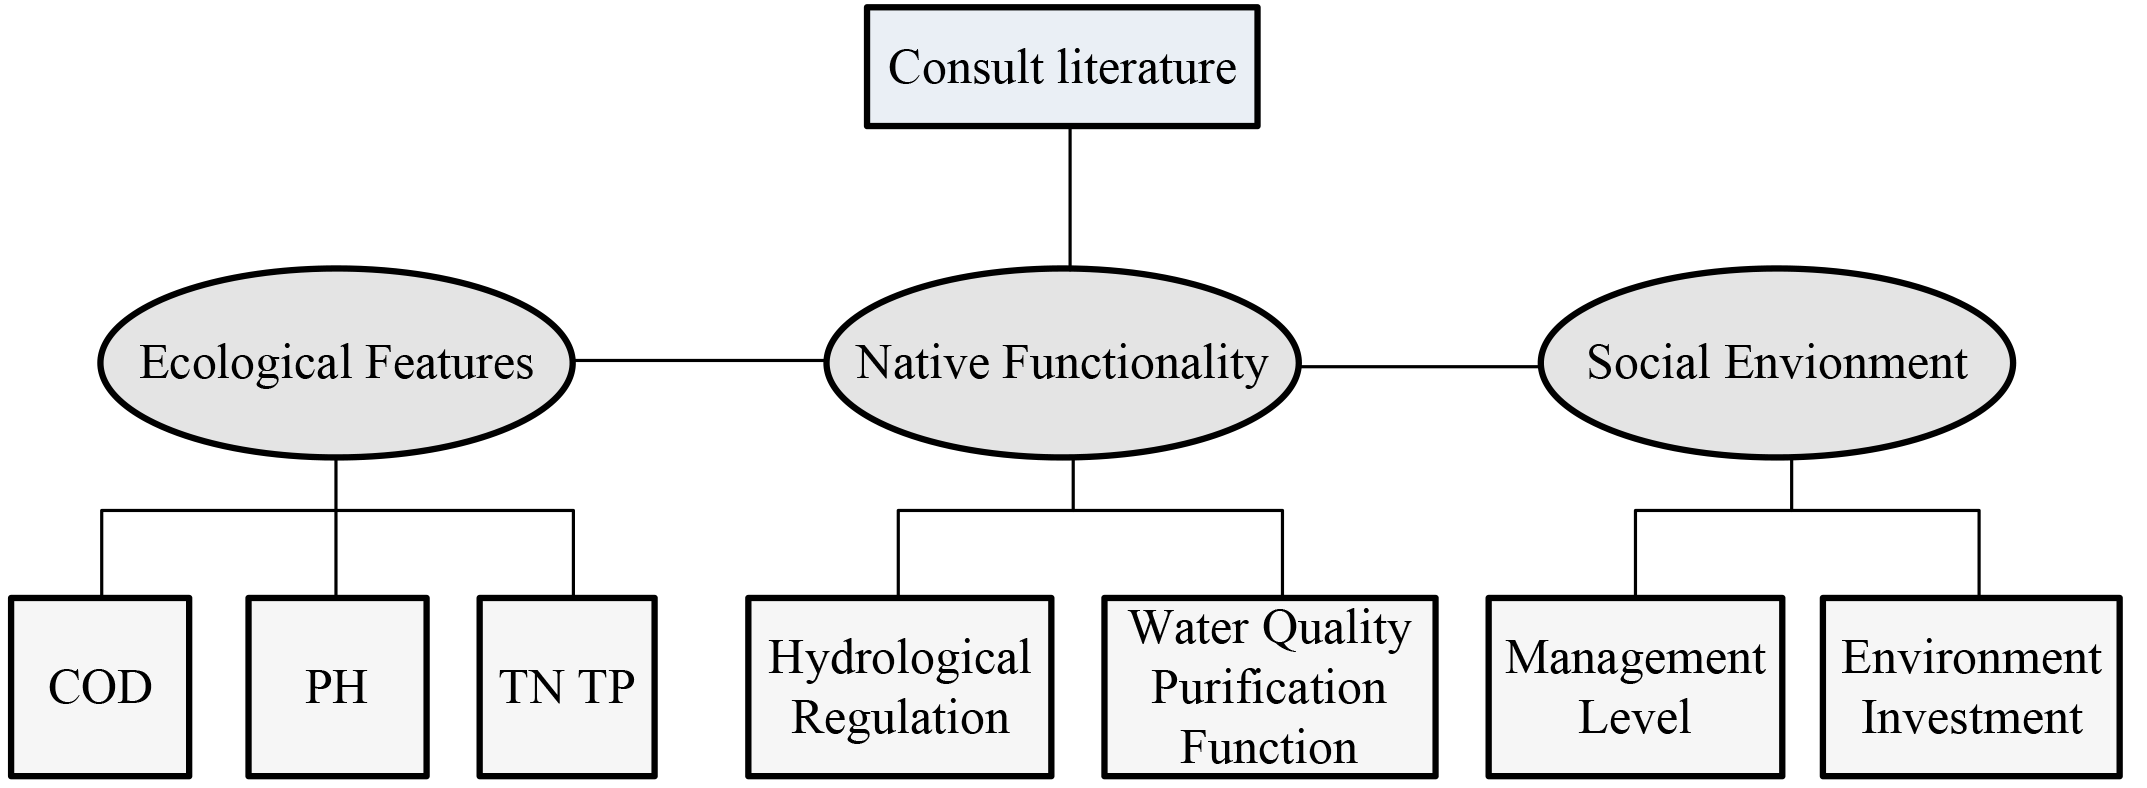
\includegraphics[width=0.7\linewidth]{figure/figure1}\\
    \captionof{figure}{Construction of AHP Model}
}
    %构造指标间的判断矩阵
    \item Construct judgment matrix \\
    %通过当地专家采用1\~{}9标度打分,对各层因素两两间量化判断,可以得到相应的判断矩阵,结果如下图:
    We can get corresponding judgment matrix in the way of 1-9 scales to evaluate by expertise and quantifying among factors, the results can be seen from the below figure   
    
    %判断矩阵图
\begin{equation}\bordermatrix{
    ~&x_1&x_2&x_3\cr
    x_1&1&7&5\cr
    x_2&1/7&1&1/5\cr
    x_3&1/5&5&1}
\end{equation}

\begin{equation}
\bordermatrix{
    ~&x_4&x_5\cr
    x_4&1&\dfrac{1}{3}\cr
    x_5&3&1}
\end{equation}


\begin{equation}
\bordermatrix{
    ~&x_6&x_7\cr
    x_6&1&3\cr
    x_7&\dfrac{1}{3}&1}
\end{equation}


\begin{equation}
\bordermatrix{
    ~&y_1&y_2&y_3\cr
    y_1&1&3&1/2\cr
    y_2&1/3&1&1/5\cr
    y_3&2&5&1}
\end{equation}


\begin{table}[H] \renewcommand\arraystretch{1.5}
    \begin{center}
        \begin{footnotesize}
            \begin{tabular}{cccccccccc}  \hline
                $x_1$&$x_2$&$x_3$ &$x_4$&   $x_5$&$x_6$&$x_7$&$y_1$&$y_2$&$y_3$\\
                TN TP&PH   &COD   & HYR &PUR&INV&MAN&ECO&NAR&SOC \\ \hline
            \end{tabular}
        \end{footnotesize}
        \caption{\footnotesize {The description of symbols}}
    \end{center}
\end{table}

    %层次单排序一致性检验
    \item Description Consistency check of single hierarchical arrangement \\
    %定义CI为一致性指标.
    We define CI as Consistency index
    
    %公式8
    \begin{equation}CI=\!\!\frac{\lambda_{max}-n}{n-1}\end{equation}
    
    
    %公式9
    \begin{equation}CR=\frac{CI}{RI}\end{equation}
    
    %一般用CR值判断.当CR<0.1时,认为成对比较的逆对称矩阵可以接受.其中RI取值见下表:
    Generally, CR value is used to judge. when CR is less than 0.1, inverse symmetric matrices can be excepted. RI values can be seen in the following table
    
    %取值表
    \begin{table}[H] \renewcommand\arraystretch{1.5}
        \begin{center}
            \caption{\footnotesize {The values of RI}}
            \begin{footnotesize}
                \begin{tabular}{ccccccccccc}\toprule[1pt]
                    \it  n & \bf 1    &\bf 2     & \bf 3  & \bf 4   &\bf 5 & \bf 6 & \bf 7 & \bf 8 & \bf 9&\bf 10   \bigstrut\\\hline
                    \it RI & 0.00 &0.00 &0.58 &0.90&1.12&1.24&1.32&1.45&1.51&1.41\bigstrut\\\bottomrule[1pt]
                \end{tabular}
            \end{footnotesize}
        \end{center}
    \end{table}
    % 层次总排序及组合一致性检验
    \item Consistency check of total taxis of hierarchy \\
    %设上一层A包含m个因素A1,A2,,,Am.A的层次总排序权值分别为a1,,,am.下一层B包含n个因素B1,,,Bn.这些因素对于Aj的层次单排序的权值分别为b1j,,,bnj.那么,此时B层的总排序权值如下表所示:
    Level A has m indexes like A1,A2,,,Am, and the weights of A total taxis of hierarchy are a1, am. Level B includes n indexes like B1,,,Bn. Eventually, we could get the weight of B's total taxis of hierarchy which can be seen in the below according to the A level single hierarchical arrangement.

\begin{figure}[H]
    \centering
    
\includegraphics[width=1.0\linewidth]{figure/table3}
    \caption{Ranking table}
\end{figure}

    %层次总排序一致性检验为:
    We get consistency check of total taxis of hierarchy
    
    %    公式10
    \begin{equation}
    CR=\displaystyle\frac{\sum\limits_{j=1}^{m}a_jCI_j}{\sum\limits_{j=1}^{m}a_jRI_j}
    \end{equation}
    
    %当CR<0.1时,认为层次总排序的结果具有满意的一致性.
    When $CR < 0.1$, the results of total taxis of hierarchy are satisfying
\end{itemize}
At last, we can get:\par

%公式11
\begin{equation}
Z=-0.2172x_1+0.0231x_2+0.0685x_3-0.0272x_4+0.0818x_5+0.4365x_6+0.1455x_7
\end{equation}\par

%5.2评价体系的建立
\subsection{The construction of evaluation system }
%对于上面得到的评价模型,我们将各项指标都取得最有值.此时得到的结果作为最好情况.我们规定此时为一级.然后,将各个指标取最坏值.我们此时得到的结果为最坏情况.我们规定此时为六级.我们将最好情况到最坏情况评价分为六部分.
We fetch optimal values from all indicators as the best condition for the evaluation model. We define this condition as the first level. On the contrary, the worst condition can be got and defined as six-level, so the condition can be divided into six levels.

%6 模型的应用
\section{Application of the Model}
%6.1 评价模型在巢湖的应用
\subsection{The application of evaluation model in Chao Hu}
%6.11巢湖评价体系的建立
\subsubsection{The construction of evaluation system on Chao Hu}
%我们收集巢湖各评价指标最优值如下表:
We collect the best values of evaluation index as follow
%    \begin{table}

%        \caption{各指标最优值表}
%   \end{table}
%带入模型,得到最优值为
Plugging values into model, we obtain the best evaluation value: 0.5\par
%同理,得到最差值为:
In the same way , the worst evaluation value is: 0.0\par
%所以,得到评价体系分级如下所示:
Evaluation system can be divided as shown below:

%分级表格
\begin{table}[H] \renewcommand\arraystretch{1.5}
    \begin{center}
        \begin{footnotesize}
            \begin{tabular}{cccccc}\toprule[1pt]
                \it Range of Evaulation value&$0.5\sim0.4$&$0.4\sim 0.3$&$0.3\sim0.2$&$0.2\sim0.1$&$0.1\sim0$\\\hline
                \it Level&1&2&3&4&5\\\bottomrule[1pt]
            \end{tabular}
        \end{footnotesize}
        \caption{\footnotesize {The criterion of evaluation}}
    \end{center}
\end{table}\par

%6.12 确定巢湖评价等级
\subsubsection{Determine evaluation grade on Chao Hu}
%我们收集的巢湖各项指标数据如下表所示:
The target data we collect are described in the following table:

%数据表
\begin{table}[H] \renewcommand\arraystretch{1.5}
    \begin{center}
        \caption{\footnotesize {Symbols Used in This Section}}
        \begin{footnotesize}
            \begin{tabular}{ccccccccc}\\\toprule[1pt]
                Index    &TN,TP&COD&PH&HYD&PUR&INV&MAN\\\hline
                Value    &$0.6$&$0.5$&$0.7$&$0.4$&$0.3$&$0.6$&$0.5$&\\\bottomrule[1pt]  
            \end{tabular}%
        \end{footnotesize}
    \end{center}
\end{table}
%带入模型得到评价值为:  
%所以属于X级
Then we get evaluation value 0.277, so it belongs to \uppercase\expandafter{\romannumeral3}.\par

%6.13结果分析
\subsubsection{Results Analysis}
%结合实际,提出一些改进措施;\par
As we know from the results of AHP, the social environmental indicator's weight is biggest. The second is the ecological index. According to our evaluation system, the level of Chao Hu is Ⅲ. It must be caused by ecological indexes. Local government and environmental administration should take some actions to improve the status of the Chao Hu. For example , manage the land-use reasonably in the watershed and reducing the emissions of N、P. From the point of land-use, increasing the area of the forest and grassland and reducing the area of plowland also can improve the status greatly.\par

%6.2预测模型在巢湖的应用
\subsection{The application of forecast model in Chao Hu}

%6.21水质变化预测
\subsubsection{Water quality change prediction}
%巢湖流域各种类型土地及输出系数结果如下表:
Land use types and export coefficient of Chao Hu catchment are shown in the below:

%巢湖流域各种类型土地及输出系数c
\begin{table}[H] \renewcommand\arraystretch{1.5}
    \begin{center}
        \caption{\footnotesize {The loads of N and P in different land use  }}
        \begin{footnotesize}
            \begin{tabular}{cccccc}\toprule[1pt]
                \bf Types&Grass Land&Urban Land&Brushwood&Dry Land&Wasteland           \\\hline
                \bf TN   &$16.86$     &$16.02$           &$10.5$   &$24.19$&$18.15$    \\
                \bf TP   &$3.2$       &$4.54$            &$2.33$   &$2.71$ &$3.25$   \\  \hline
                \bf Types&Dry Land  &Residential Land    &Wetland  &Water  &Paddy Field        \\
                \bf TN   &$13.9$      &$20.98$           &$2.16$   &$0$    &$26.21$    \\
                \bf TP   &$2.64$      &$4.53$            &$0.9$    &$0$    &$3.28$     \\\bottomrule[1pt]
            \end{tabular}
        \end{footnotesize}
    \end{center}
\end{table}
\vspace{-0.5cm}
As we can know from the table six, the load of TN of the unit area non-point source of various land-use is $0~26.21mg/L$ and the load of TN of the unit area non-point source of various land-use is $0~4.54mg/L$. The paddy field and dry farm's load of unit area TN are the highest. The rural resident and urban land-use's load of unit area TP are the highest. The reason of the above situation might be the cause we give as following:
\begin{enumerate}
    \item The daily sewage of rural-urban fringe zone and the area of plow are expanding in the Chao Hu watershed.
    \item The scale of livestock farming increase.\\
    According to the above table seven, we can see that the TN、TP discharge of the paddy field is the highest. Causing the result is because of the percentage of paddy field that is large. With the development of society, the area of urban land-use is increasing and the area of rural resident and dry farm are reducing.
    
\end{enumerate}
\par

%6.22赤潮发生预测
\subsubsection{The forecast of potentially-toxic algal blooms reproduction}
%我们收集巢湖相关的数据共129组,对数据进行分配,其中91组作为训练数据,19组作为验证数据,19组作为测试数据,训练18代后结果收敛,得到的训练效果曲线如下:
We collect relevant data about Chao Hu from 129 groups, which are assigned subsequently, and 91 groups are used as train data, 19 groups as validation data and 19 groups as train data, The results converge reasonably well when data are trained at the 18 generation and the effects of curve is shown as follows:\\

%训练效果曲线
\begin{figure}[H]
\centering
\includegraphics[width=0.7\linewidth]{"figure/TrainingPerformance"}
\caption{Training Performance}
\end{figure}

%相关系数曲线如下:
The correlation coefficient curve as follow:\\
%相关系数曲线
\begin{figure}[H]
\centering
\includegraphics[width=0.7\linewidth]{figure/Regression}
\caption{Regression}
\end{figure}

%结果分析:最终训练出来的模型与实际数据相关性达到了91%,说明神经网络拟合效果很好,符合我们对N,P含量对叶绿素a含量影响的预期表现.
Analysis result, the correlation between the model trained with data and real data is up to 91\%,reflecting that BP neutral network method is feasible to predict .the N,P concentrations have a great impact on the quantity of chlorophyll a and getting a better outcome.\par

%也就是说,N,P含量之间影响到了水中藻类的生长,经过统计与预测,当N含量大于2.5mg/L,P含量大于0.3mg/L时便可能使叶绿素a超标,产生水华,并且在实际水藻的生长环境允许范围内,叶绿素a含量随着N,P含量的增长而增长,也就意味着水中藻类数量在增加。
That's to say, the growth of potentially-toxic algal blooms in water is affected by N,P nutrient load, by statistics analysis and prediction, potentially-toxic algal blooms will reproduce in water when nitrogen content exceed 2.5mg/L and nitrogen content is bigger than 0.3mol/L, furthermore, chlorophyll a content will increase with increasing N,P nutrient load.\par 

\section{The sensitivity analysis of the evaluation model}
We only consider seven evaluating indexes to evaluate a lake in our evaluation model. Obviously, these indicators are incomplete. As for the other indicators, we assume that they are all at the optimal conditions. But actual situation is not always like what we assume. We test the sensitivity of the model with environmental awareness.\par
The environmental awareness belongs to the index system of social environment. The uncertainty of environmental awareness is large in the actual cases. We analyze the fluctuation of the result under different environmental awareness.\par
Sensitivity calculation results are as follows:

%公式11
\begin{equation}
S(z,x_e)=\frac{dz}{dx_{e}}\cdot\frac{x_e}{z}=-3.06
\end{equation}

As we can see from the results, evaluation model is greatly influenced by environmental awareness. The reason for this result may be that the environmental awareness influences some indexes. What's more, stability of our model also need to be further improved.\par

\section{Model evaluation}
\subsection{Strengths}
The export coefficient model based on hydrology needs few parameters and its operation is simple. Not only does it have a comprehensive consideration but also certain accuracy.\par
We use the BP neural net model to forecast the Water quality and potentially-toxic algal blooms, avoiding analyzing the complex relationship between various factors.\par
Given the factors including ecology、nature and society, the model of evaluation with the AHP can integrability evaluate a lake.\par
\subsection{Weaknesses}
Lack of Data Support: the data for the problem is hard to get. The data we collect are little for the model we build.\par
Estimated Parameters: Due to lack of data, some values used in the calculations had to be estimated.\par
Simplified Assumption: Simplifying assumptions had to be made in order to create a solvable model.\par
\subsection{Future Work}
Because the system of evaluation of the lake is very complex. Only seven indexes can not make it clear. Our evaluating model needs more indexes to be perfect. What's more, we should combine the AHP with the Fuzzy Algorithm rather than only the AHP to make the model of evaluation more reasonable. We should collect more data for the model to improve the stability of the model.\par

\newpage
\begin{thebibliography}{99}
    \bibitem{1} Omernik J M. The influence of land use on stream nutrient levels[ R]. New York: USEPA Corvallis, OR, 1976\label{1}
    \bibitem{2}Nielsen H. Komogorovs mapping neural network existence theorem[C]\\\\Proceedings of the International Confereneeon Neural Networks.New York:IEEE Press.1987.1(3):11—13.\label{2}
    \bibitem{3}Michele S,Lawrence W.Harding JR.Developing an empirical model of phytoplankton primary production:a neural network case study[J].Ecological Modeling,1999,120(59):213—223. \label{3}
    
\end{thebibliography}
\end{document}
